\section{Θυρίδες Βαθιάς Συχνοτικής/Χωρικής Αποσυσχέτισης και Κωδικοποίησης}
\par
    To δίκτυο της \enit{3D} κωδικοποίησης μέσω νευρωνικών θυρίδων Fourier. Συνδυάζει τις παραπάνω μεθόδους κωδικοποίησης σε ένα ολοκληρωμένο δίκτυο το οποίο αποσυσχετίζει συχνοτικά τον τρισδιάστατο χώρο σε υψηλής και χαμηλής συχνότητας χαρακτηριστικά με το σκεπτικό του μετασχηματισμού κυματιδίων (\enit{Wavelet Transform}). 
\par    
    Η ιδέα προήλθε απο το κείμενο της έρευνας \enit{Neural Fourier Filter Banks} \cite{wu2023neural}. Κατεύθυνση της ιδέας είναι να αξιοποιήσει την χωρική διαμέριση που προσφέρει η νευρωνική κωδικοποίηση \enit{Multi-Resolution Hash Encoding} και να κωδικοποιήσει τα υψηλής διάστασης χαρακτηριστικά ξεχωριστά σε κάθε διαμέριση με συχνοτικούς μετασχηματισμούς ανάλογους του \enit{Positional Encoding}. Έτσι το νευρωνικό δίκτυο αναπαριστά φίλτρα χαμηλών και υψηλών συχνοτήτων τα οποία αντιστοιχίζουν με αυτό τον τρόπο τις συντεταγμένες σε ειδικές δομές που λέγονται \enit{Fourier Grid Features} και με αυτόν τον τρόπο επιτρέπεται καλύτερος εντοπισμός στην κλίμακα αλλά και στην συχνότητα βαθιών \enit{SDF} χαρακτηριστικών. 
\par
    H διαδικασία περιλαμβάνει την μετατροπή των  \enit{Grid Features} (κεφ.\ref{section4:NeuralHashGridEncoding}) σε \enit{Fourier Features} εφαρμόζοντας τον μετασχηματισμό Fourier  μέσω συναρτήσεων πυρήνα που περιγράφτηκε στο κεφάλαιο \ref{section4:FourierFeatureNets}. 
    Ταυτόχρονα για την διατήρηση της υψηλοσυχνοτικής πληροφορίας χρησιμοιείται συμπληρωματικό πλήρως συνδεδεμένο δίκτυο με ημιτονοειδή συναρτήσεις που οδηγεί τα χαμηλοσυχνοτικά και υψηλοσυχνοτικά χαρακτηριστικά (ανάλογο του \enit{SIREN} δικτύου). 
    \clearpage
\par 
    Η συνολική μορφή που παίρνει το δίκτυο \enit{IDR}  μπορεί να αποδοθεί με το παρακάτω διάγραμμα. 
    \begin{figure}[ht]
        \centering
        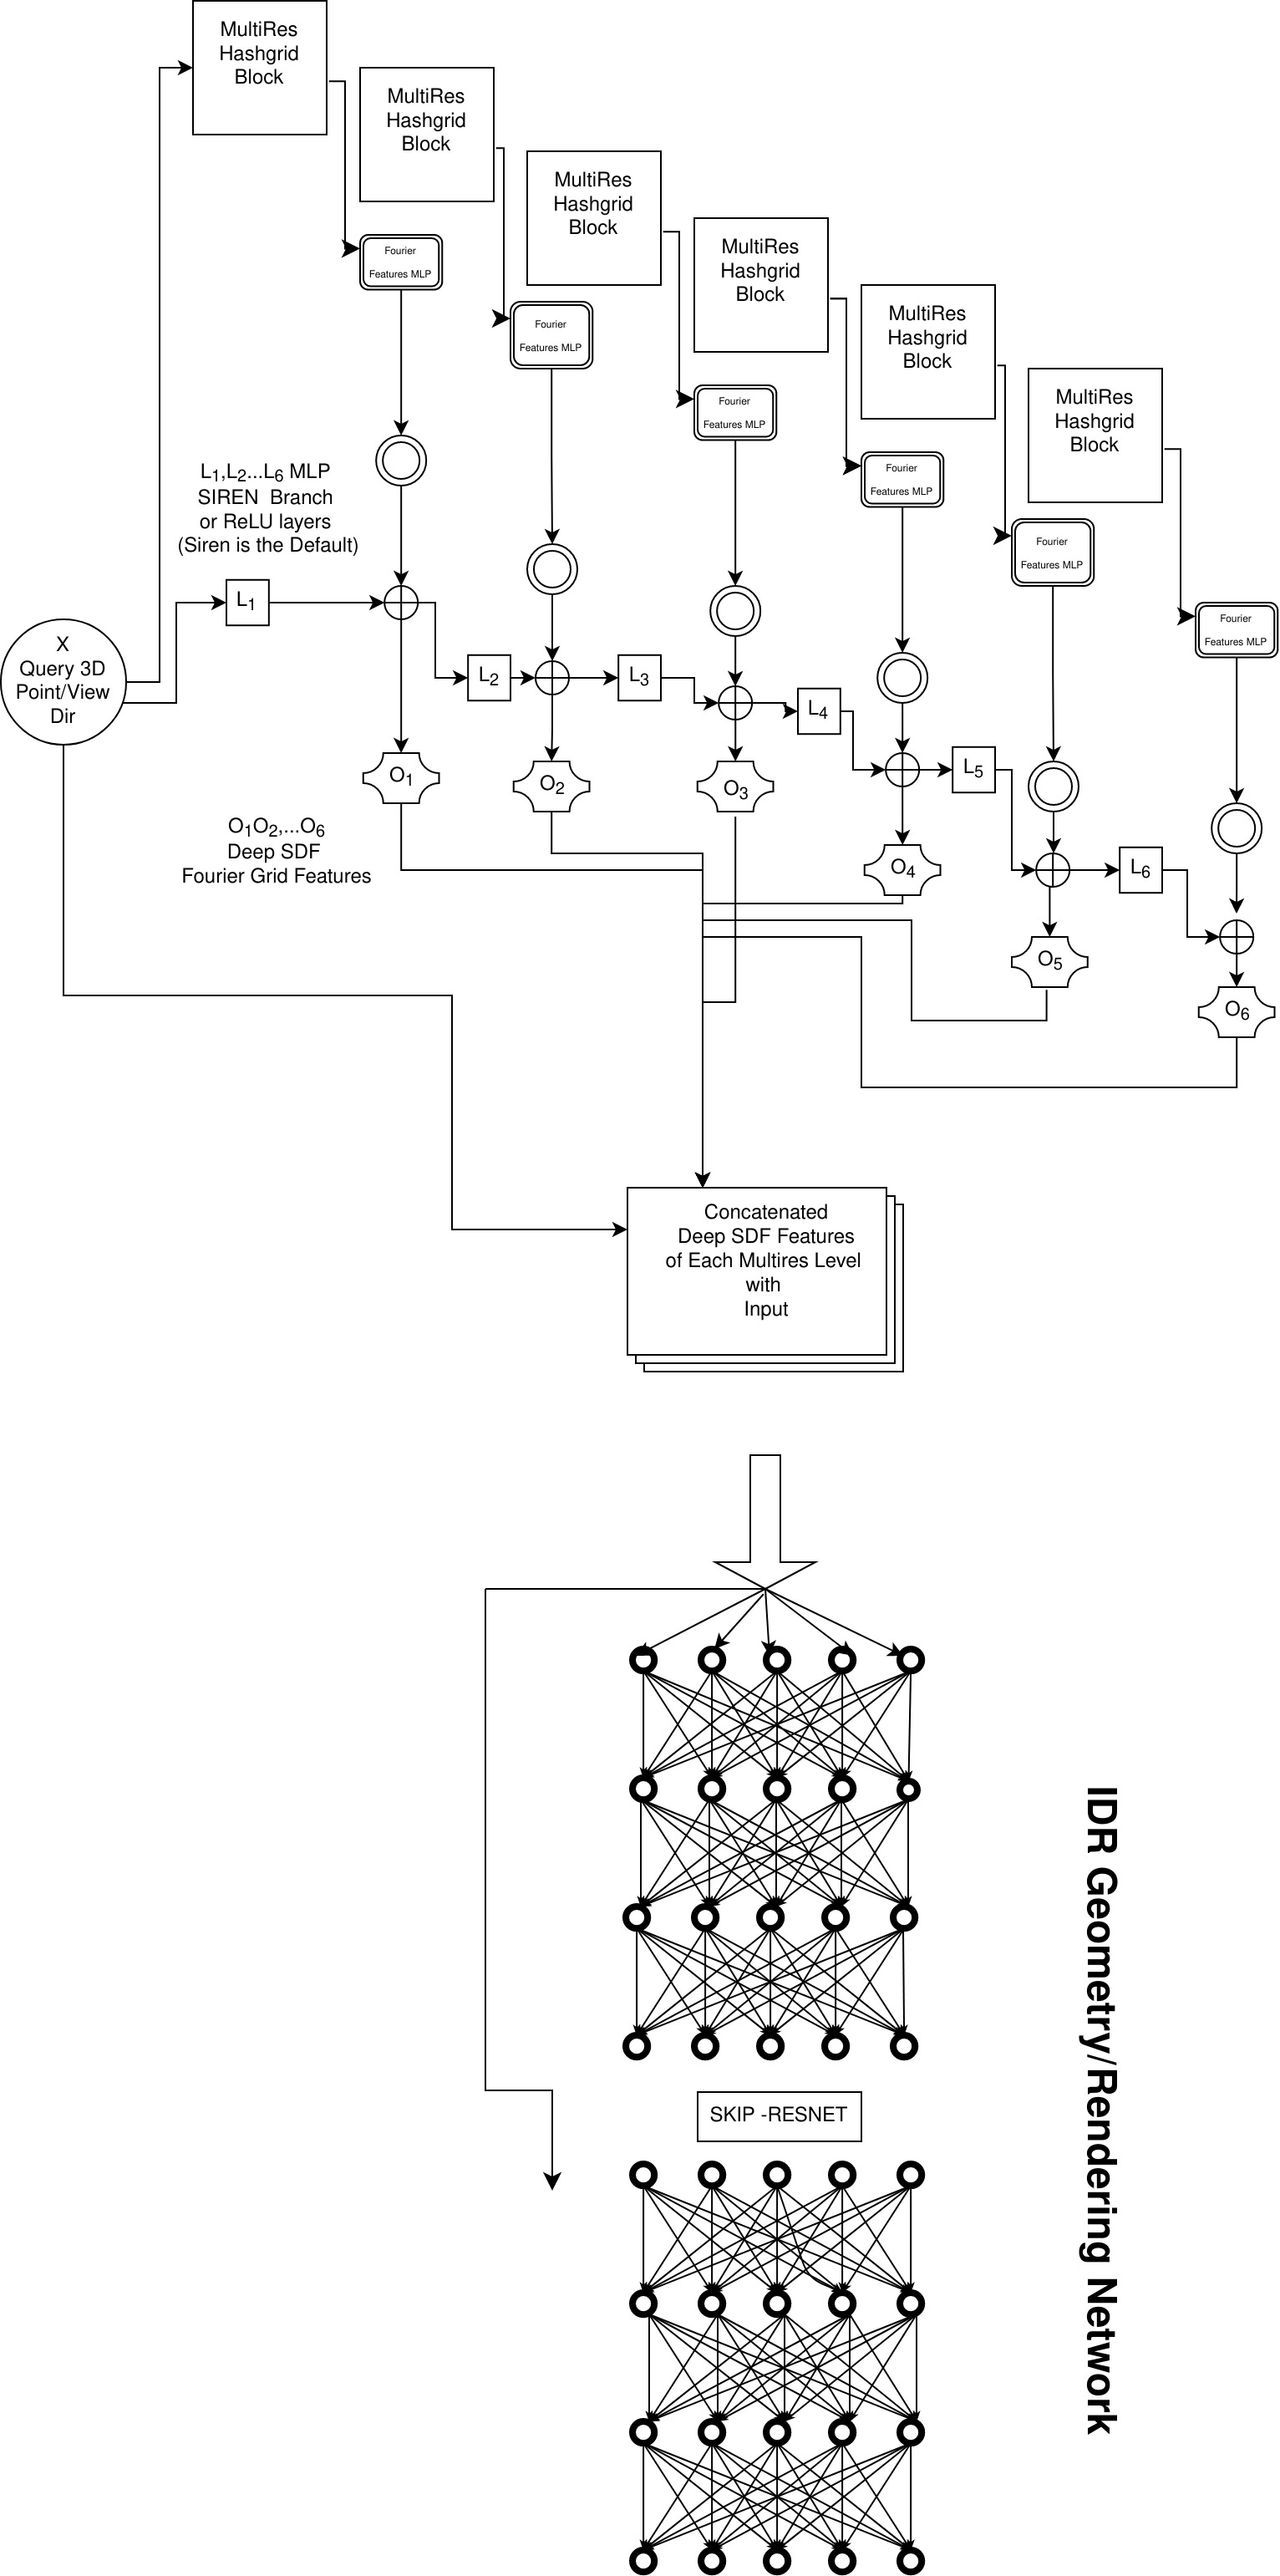
\includegraphics[height=0.72\textheight]{images/chapter4_img/IDR_Embeddings_Architecture-Neural Fourier Filter Banks.jpg}
        \caption{Αρχιτεκτονική δικτύου 3D Κωδικοποίησης NFFB}
        \label{fig:nffbarchitecture}
    \end{figure}
    \clearpage
